\documentclass[12pt, a4paper]{article}
\usepackage{kinebot}
\usepackage{booktabs}
\usepackage{array}
\usepackage{float}
\usepackage{placeins}
\usepackage{pgfplots}
\pgfplotsset{compat=1.18}
\pgfplotsset{
  kinebotgraph/.style={
    ybar,
    bar width=14pt,
    width=0.92\textwidth,
    height=5cm,
    ymin=0,
    axis lines*=left,
    ymajorgrids,
    major grid style={draw=gray!25},
    enlarge x limits=0.15,
    legend columns=1,
    legend cell align=left,
    legend style={
      at={(0.5,-0.32)},
      anchor=north,
      draw=none,
      font=\small,
    },
    legend image code/.code={\draw[#1] (0cm,-0.1cm) rectangle (0.3cm,0.1cm);},
    nodes near coords,
    nodes near coords style={font=\scriptsize},
    every axis plot/.append style={draw=black, line width=0.3pt},
    x tick label style={font=\small, align=center},
  },
  kinebotbarA/.style={fill=gray!45},
  kinebotbarB/.style={fill=gray!85},
  kinebotbarC/.style={fill=gray!65},
}

\let\oldsection\section
\renewcommand{\section}{\FloatBarrier\oldsection}

% Tabelas longas (mais de ~15 linhas) usam longtable para quebrar entre páginas.
\usepackage{longtable}
\usepackage{needspace}
\setlength{\LTcapwidth}{\textwidth}

% Apêndices numerados (Apêndice 1, 2, ...). Uso: \apendices uma vez, depois
% \apendice{Título}{sec:apendice-x}. No texto: Apêndice~\ref{sec:apendice-x}.
\newcounter{apendice}
\newcommand{\apendices}{}
\newcommand{\apendice}[2]{%
  \Needspace{8\baselineskip}%
  \refstepcounter{apendice}\label{#2}%
  \section*{Apêndice \theapendice\ - #1}%
  \addcontentsline{toc}{section}{Apêndice \theapendice\ - #1}}

\reporttitle{TITULO}
\reportsubtitle{Relatório de pesquisa: SUBTITULO}
\reportauthor{Sofia Wamser Lima}
\reportdate{\today}
\reportref{v1.0}
\reportcity{Curitiba}

\begin{document}

\pagenumbering{gobble}
\makecover

\tableofcontents
\cleardoublepage

\pagenumbering{arabic}
\pagestyle{fancy}

\section{Introdução}

CONTEXTO. PERGUNTA DE PESQUISA. O QUE ESTE RELATÓRIO RESPONDE.

\section{Metodologia}

\subsection{Dados e escopo}

DADOS, CRITÉRIOS DE INCLUSÃO E EXCLUSÃO, RECORTES.

\subsection{Método adotado}

MÉTODO E POR QUE. ALTERNATIVAS DESCARTADAS:

\begin{itemize}
  \item \textit{Alternativa A}: descrição breve e motivo da rejeição.
\end{itemize}

\section{Resultados}

\subsection{ACHADO PRINCIPAL}

FRASE DE ENQUADRAMENTO.

\begin{table}[H]
\centering
\caption{DESCRIÇÃO.}
\label{tab:principal}
\begin{tabular}{lrr}
\toprule
\textbf{Categoria} & \textbf{Valor} & \textbf{\%} \\
\midrule
Item A & 000 & 00,0\% \\
\bottomrule
\end{tabular}
\end{table}

INTERPRETAÇÃO COM COMPARAÇÃO E INCERTEZA.

\begin{figure}[H]
\centering
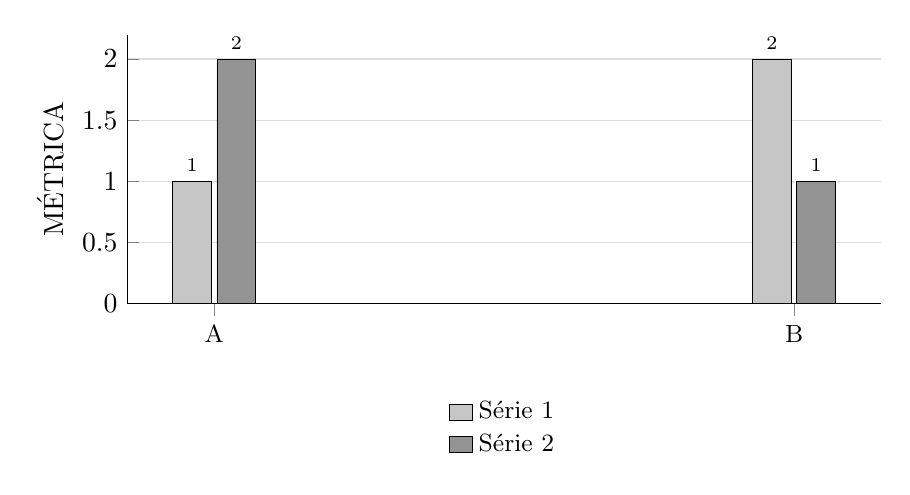
\begin{tikzpicture}
\begin{axis}[kinebotgraph, symbolic x coords={A,B}, xtick=data, ylabel={MÉTRICA}]
  \addplot[kinebotbarA] coordinates {(A,1) (B,2)};
  \addplot[kinebotbarB] coordinates {(A,2) (B,1)};
  \legend{Série 1, Série 2}
\end{axis}
\end{tikzpicture}
\caption{DESCRIÇÃO.}
\label{fig:principal}
\end{figure}

\section{Conclusão}

RESPOSTA DIRETA À PERGUNTA, COM O NÚMERO QUE MAIS IMPORTA.

Pontos em aberto:

\begin{enumerate}
  \item PONTO EM ABERTO E PRÓXIMO PASSO.
\end{enumerate}

\end{document}
